\chapter{Referencial Teórico}
\label{Referencial_Teorico}

\section{Arqueologia}%
A arqueologia é a ciência que estuda as culturas humanas através da recuperação, análise e interpretação dos vestígios materiais deixados por essas sociedades ao longo do tempo. Esses vestígios podem incluir artefatos, edificações, utensílios, entre outros elementos materiais que fornecem informações valiosas sobre os modos de vida, as práticas sociais e as organizações econômicas e políticas dos povos antigos. Conforme destaca \cite{funari2024arqueologia}, a arqueologia é essencial para a compreensão da história da humanidade, pois complementa e enriquece os dados obtidos por outras disciplinas, como a história e a antropologia, permitindo uma visão mais abrangente e detalhada das sociedades passadas. Assim, ao explorar os vestígios materiais, os arqueólogos contribuem significativamente para a reconstrução e preservação da memória coletiva, além de promover a valorização do patrimônio cultural.
Ao falar de arqueologia podemos nos deparar com várias formas de expressão, como por exemplo, a arte rupestre.
\subsection{Arte Rupestre}
%Falar sobre a definição(que é mais geral), falar sobre a toca da onça. sobre pictoglifos(que são as pinturas).



O termo “rupestre” tem origem no latim "rupestris”, derivado de “rupes”, que significa "rocha" ou “penhasco”. Assim, define-se como "Arte Rupestre” toda expressão gráfica, seja gravura ou pintura, que utiliza como suporte uma superfície rochosa, independentemente de suas características e dimensões \cite[p. 7]{pedroignacioschmitz_1984_arte}. As paredes de abrigos, grutas, penhascos e até mesmo rochas isoladas se transformam em telas para essas manifestações ancestrais.
Existem dois principais tipos de arte rupestre:
\begin{itemize}
\item \textbf{Pintura Rupestre (Pictografia):} Criação de imagens utilizando pigmentos minerais, vegetais ou animais, aplicados diretamente na superfície rochosa.
\item \textbf{Gravura Rupestre (Petróglifo):} Produção de desenhos através do desgaste da superfície rochosa, utilizando ferramentas líticas, como pedras pontiagudas.
\end{itemize}
A arte rupestre, presente em diversas partes do mundo, representa uma das formas mais antigas de expressão humana, oferecendo informações valiosas sobre as culturas que as produziram (MARQUES, 2016).

\subsection {Sítio Arqueológico Lapa da Pedra}
O Sítio Arqueológico Lapa da Pedra, conforme mostrado na Figura \ref{fig:Entrada da Gruta IV,Toca da Onça}, é conhecido popularmente como Toca da Onça. Em 1984, Pedro Ignácio Schmitz e Altair Sales Barbosa realizaram pesquisas que culminaram na identificação e catalogação de 29 pequenas grutas na região de Formosa, Goiás. Essas grutas abrigavam pinturas rupestres e serviram como moradia para os primeiros habitantes do cerrado (BARBOSA et al., 1984, 1993).
Dentre as 29 grutas, a Gruta catalogada por Schmitz como IV–GO-EC-002 (04), se destaca pela maior concentração de pictoglifos e, portanto, \textbf{foi o foco da virtualização neste trabalho}. Localizada a cerca de 12 km da cidade de Formosa, a Gruta 04 consiste em uma passagem de duzentos metros abaixo de uma enorme pedra calcária, situada na fazenda Pedra. Esse sítio, semelhante a outros em Goiás e no noroeste de Minas Gerais, apresenta uma grande diversidade de temas na arte rupestre, datando de aproximadamente 4.560 a.C. (SCHMITZ, 1990).


\begin{figure}[H]
    \centering
    \includegraphics[height=11cm, keepaspectratio]{img/Entrada Gruta IV Toca da Onça.jpeg}
    \caption{Entrada da Gruta IV, Toca da Onça. \\
        \textbf{Fonte:} Autoria Própria.}
    \label{fig:Entrada da Gruta IV,Toca da Onça}
\end{figure}



\subsection{Ameaças à Preservação da Arte Rupestre: Deteriorização e Ação Antrópica}
A arte rupestre, como patrimônio cultural de valor \textbf{inestimável}, enfrenta diversos desafios para sua preservação. A ação do tempo e as condições climáticas, como a umidade, a luz, o calor e o vento, contribuem para a deterioração natural das pinturas e superfícies rochosas.
Na Toca da Onça,  não bate sol dentro da gruta, contribuindo para a preservação do estado dos desenhos. Contudo, ainda se observam fatores de deterioração natural: descamação da tinta, infiltrações, fissuras nas rochas.


Além da deterioração natural, a ação antrópica, que se configura como a interferência humana no ambiente, representa uma grave ameaça à preservação da arte rupestre. Vandalismo, turismo desordenado, contato direto com as pinturas, poluição e obras próximas aos sítios arqueológicos podem causar danos irreversíveis a este patrimônio.
Em relação à Toca da Onça, os seguintes exemplos de impactos causados pela ação antrópica foram notados: vandalismo, pichações, degradação causada pelo turismo desordenado, fotos com \textit{flash}. Como por exemplo o que pode ser observado na Figura \ref{fig:degradacao_toca_onca}.

\begin{figure}[H]
    \centering
    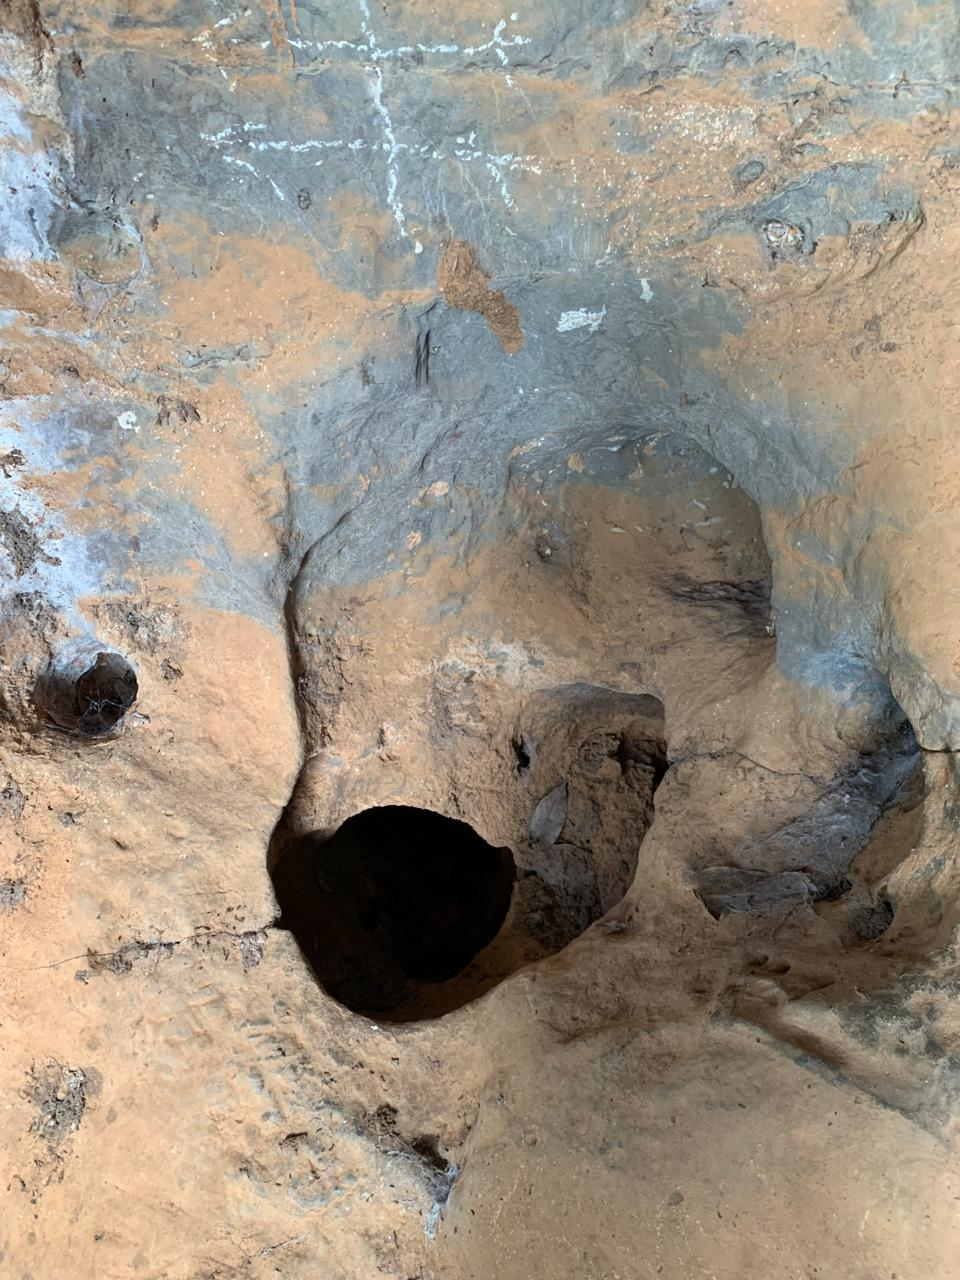
\includegraphics[height=11cm, keepaspectratio]{img/jogo da velha.jpeg}
    \caption{Depredação do Patrimônio na Toca da Onça. \\
        \textbf{Fonte:} Autoria Própria.}
    \label{fig:degradacao_toca_onca}
\end{figure}


\section{Patrimônio Virtual (Virtual Heritage)}
\subsection{Conceitos e Importância}
Discutir o conceito de patrimônio virtual e seu impacto na arqueologia.

Diante dos desafios para a preservação da arte rupestre, a virtualização 3D surge como uma ferramenta poderosa para documentar, estudar e divulgar este importante patrimônio cultural, minimizando os impactos causasdos da visitação aos sítios arqueológicos.

\subsection{Aplicações em Arqueologia}
Dar exemplos de como o patrimônio virtual tem sido usado para preservar sítios históricos.




\section{Fotogrametria e Modelagem 3D}
Para construção de um Patrimônio Virtual com qualidade é preciso construir modelos 3D fidedignos a realidade e para isso existe uma técnica muito utilizada chamada fotogrametria.
A fotogrametria, deriva das raízes gregas “photós” (luz), “gramma” (desenhado ou escrito) e “metria” (medição). Logo, fotogrametria etimologicamente significa “medições gráficas por meio da luz" (Paredes, 1987). A American Society for Photogrammetry and Remote Sensing (ASPRS), em seu livro The Manual of Photogrammetry (2003), define fotogrametria como “a arte, ciência e tecnologia de obter informações confiáveis sobre objetos físicos e o ambiente por meio de processos de registro, medição e interpretação de imagens fotográficas e padrões de energia radiante eletromagnética (EM) e outros fenômenos.”
Historicamente, a fotogrametria  teve seu desenvolvimento intrinsecamente ligado à evolução da fotografia, da óptica e da geometria, culminando em uma ferramenta crucial para diversos campos do conhecimento. No Brasil, sua história acompanha de perto a evolução global, com momentos de pioneirismo e adaptação às demandas nacionais (Silva, 2015).

Quanto a sua evolução, a fotogrametria passou por quatro fases principais: a Fotogrametria de Tábua Plana (1850–1900), iniciada por A. Laussedat com o uso de fotografias terrestres para mapeamento (Silva e Borges, 2023); a Fotogrametria Analógica (1900–1950), que incorporou a estereoscopia e fotografias aéreas para fins topográficos; a Fotogrametria Analítica (1950-1990), que otimizou os processos com a introdução de computadores e automatização; e a Fotogrametria Digital (1990-atualmente), caracterizada por processos automáticos realizados em computadores, além da popularização de câmeras digitais de alta qualidade que simplificam o processo (Borges e Silva, 2023).

A criação de um modelo 3D com fotogrametria digital, como descrito por Linhares e Groetelaars (2021), envolve um processo que se inicia com o planejamento do levantamento, definindo os objetivos, escolhendo o equipamento adequado e planejando a tomada fotográfica. A etapa seguinte, como apresentado por Groetelaars (2004), é a aquisição de dados no campo, que consiste na captura de fotografias e na medição das coordenadas dos pontos de controle no espaço real, utilizando métodos topográficos ou 3D Laser Scanning. Após a aquisição, o processamento dos dados é realizado por softwares específicos, que orientam as imagens interna e externamente com base nos pontos de controle, gerando uma nuvem de pontos densa. A partir dessa nuvem, o software cria uma malha triangular irregular (TIN), que representa a forma do objeto e pode ser texturizada com as imagens originais. A etapa final envolve o pós-processamento para remover ruídos, \textit{outliers} e falhas, otimizar a malha e aplicar texturas, resultando em um modelo 3D fotorrealístico.
A fotogrametria automatizada, comumente empregada na geração de modelos 3D de sítios arqueológicos, envolve um processo que se inicia com a captura de imagens de alta qualidade, utilizando câmeras terrestres ou aéreas com sobreposição e georreferenciamento por meio de pontos de controle (GCPs) (McGlone, 2004). O software realiza o alinhamento das imagens, corrigindo distorções geométricas e determinando a posição e orientação de cada fotografia no espaço. Através da correlação de imagens, o software identifica pontos correspondentes e calcula as coordenadas 3D de cada ponto, gerando uma nuvem densa de pontos 3D (Heipke, 2001). A partir da nuvem de pontos, o software gera modelos 3D, atribui texturas e corrige distorções geométricas, produzindo modelos 3D precisos e realistas do sítio arqueológico (Gruen, 2008). A geração de modelos 3D permite a documentação detalhada do sítio, a análise tridimensional da estrutura e a criação de representações visuais para estudos e divulgação científica.


%\subsection{Engine}
\subsection{Unreal Engine}No contexto do desenvolvimento de jogos e aplicações interativas, a \textit{engine} desempenha um papel fundamental como a espinha dorsal tecnológica. Uma \textit{engine} de jogo é um conjunto complexo de bibliotecas de software que fornece aos desenvolvedores um arcabouço completo para criar e alimentar experiências interativas em tempo real. Essas ferramentas abrangem desde a renderização gráfica e simulação de física até a inteligência artificial, interface do usuário e gerenciamento de áudio. Sem uma \textit{engine}, os desenvolvedores precisariam construir todas essas funcionalidades do zero, tornando o processo de desenvolvimento significativamente mais complexo e demorado. 

A \textit{Unreal Engine}, desenvolvida pela\textit{ Epic Games}, se destaca como uma \textit{engine} de jogos de última geração, amplamente utilizada na indústria de jogos e simulações, e reconhecida por sua capacidade de criar experiências visuais de alta qualidade e interativas.  A \textit{Unreal Engine} oferece um conjunto robusto de ferramentas para modelagem 3D, animação, física, renderização, iluminação, realidade virtual e muito mais. Sua arquitetura flexível e código-fonte aberto permitem que os desenvolvedores personalizem e estendam a \textit{engine} para atender às necessidades específicas de seus projetos, tornando-a uma escolha popular tanto para grandes estúdios quanto para desenvolvedores independentes.

No âmbito do Patrimônio Virtual, a \textit{Unreal Engine} se torna uma ferramenta poderosa para a criação de reconstruções digitais imersivas e interativas de sítios arqueológicos, monumentos e artefatos históricos. A \textit{engine} permite a modelagem 3D realista, a aplicação de texturas detalhadas e a simulação precisa de iluminação, proporcionando aos usuários uma experiência virtual imersiva e próxima da realidade. A capacidade de integrar elementos interativos, como navegação em primeira pessoa, animações e informações contextuais, enriquece ainda mais a experiência, tornando a \textit{Unreal Engine} uma escolha estratégica para projetos que buscam aproximar o público do patrimônio cultural de forma inovadora e envolvente.
\begin{figure}[H]
    \centering
    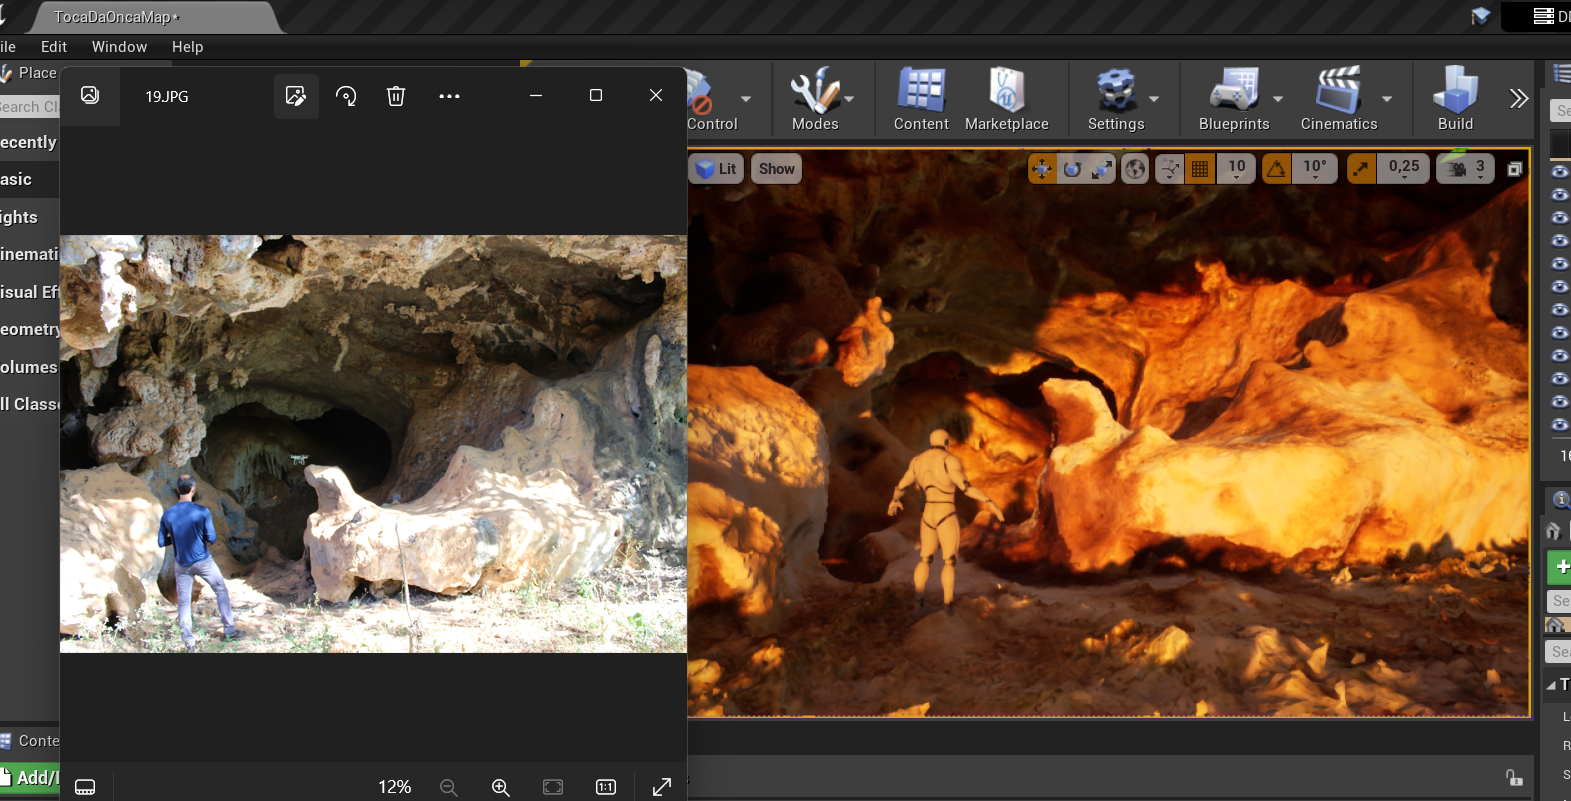
\includegraphics[height=6cm, keepaspectratio]{img/unreal-print.png}
    \caption{Calma Afrânio, eu vou pensar num nome e pegar uma foto melhor \\
    \textbf{Fonte:} Autoria Própria.}
    \label{fig:unreal-print}
\end{figure}
To colocando aqui só pra deixar a estrutura pronta e lembrar de colocar imagem.
Quanto mais imagem, mais rico o trabalho fica. Com a estrutura feita, depois é só eu trocar o arquivo.
\begin{figure}[H]
    \centering
    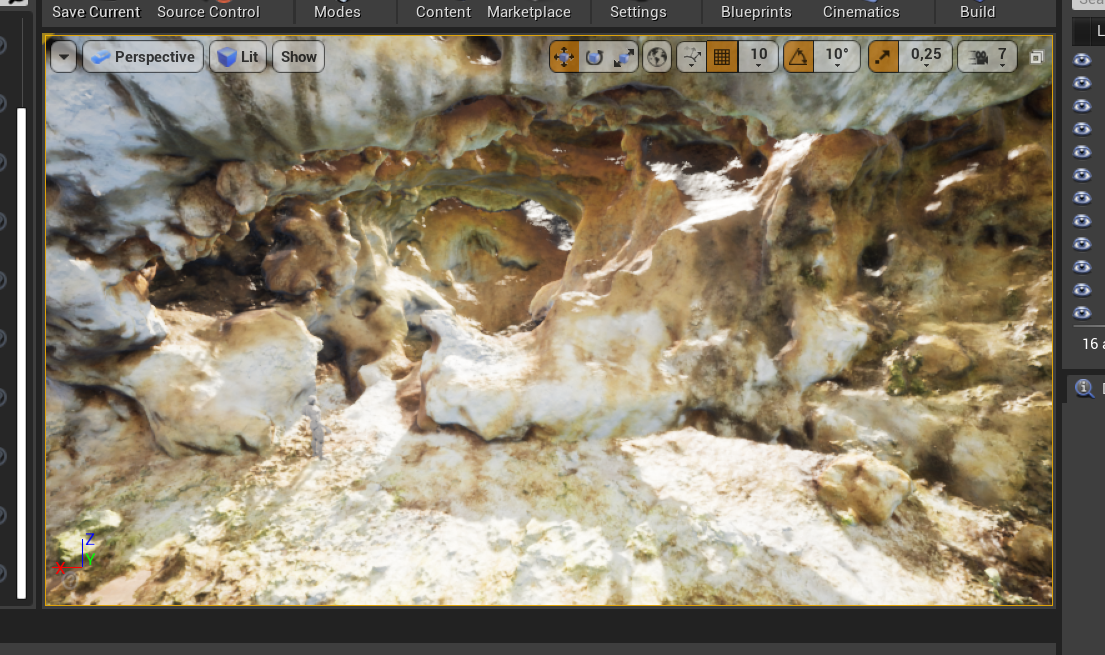
\includegraphics[height=8cm, keepaspectratio]{img/unreal-print2.png}
    \caption{UnrealEngine.}
    \label{fig:unreal-print2}
\end{figure}
\subsection{Metahumans}

A representação humana em ambientes virtuais tem papel crucial na criação de experiências imersivas e relacionáveis. No contexto do Patrimônio Virtual, a presença de personagens virtuais humanoides pode auxiliar na comunicação de narrativas históricas, guiar usuários por sítios arqueológicos reconstruídos e demonstrar costumes e atividades do passado. Nesse sentido, a ferramenta \textit{MetaHuman Creator} (Figura \ref{fig:metahuman creator}), da Epic Games, surge como um recurso poderoso para a criação de avatares digitais de alta fidelidade.
O \textit{MetaHuman Creator} permite a geração e personalização de rostos e corpos humanos com alto nível de realismo, incluindo detalhes como textura de pele, cabelo, expressões faciais e diferentes tipos de corpo. A interface intuitiva e a ampla gama de opções de personalização permitem a criação de personagens únicos e específicos, evitando a aparência genérica frequentemente associada a avatares digitais. Esse recurso permite a criação detalhada de personagens realistas que podem ser integrados em simulações e experiências interativas, enriquecendo a representação do patrimônio cultural, tornando-a mais próxima e humanizada.

\begin{figure}[H]
    \centering
    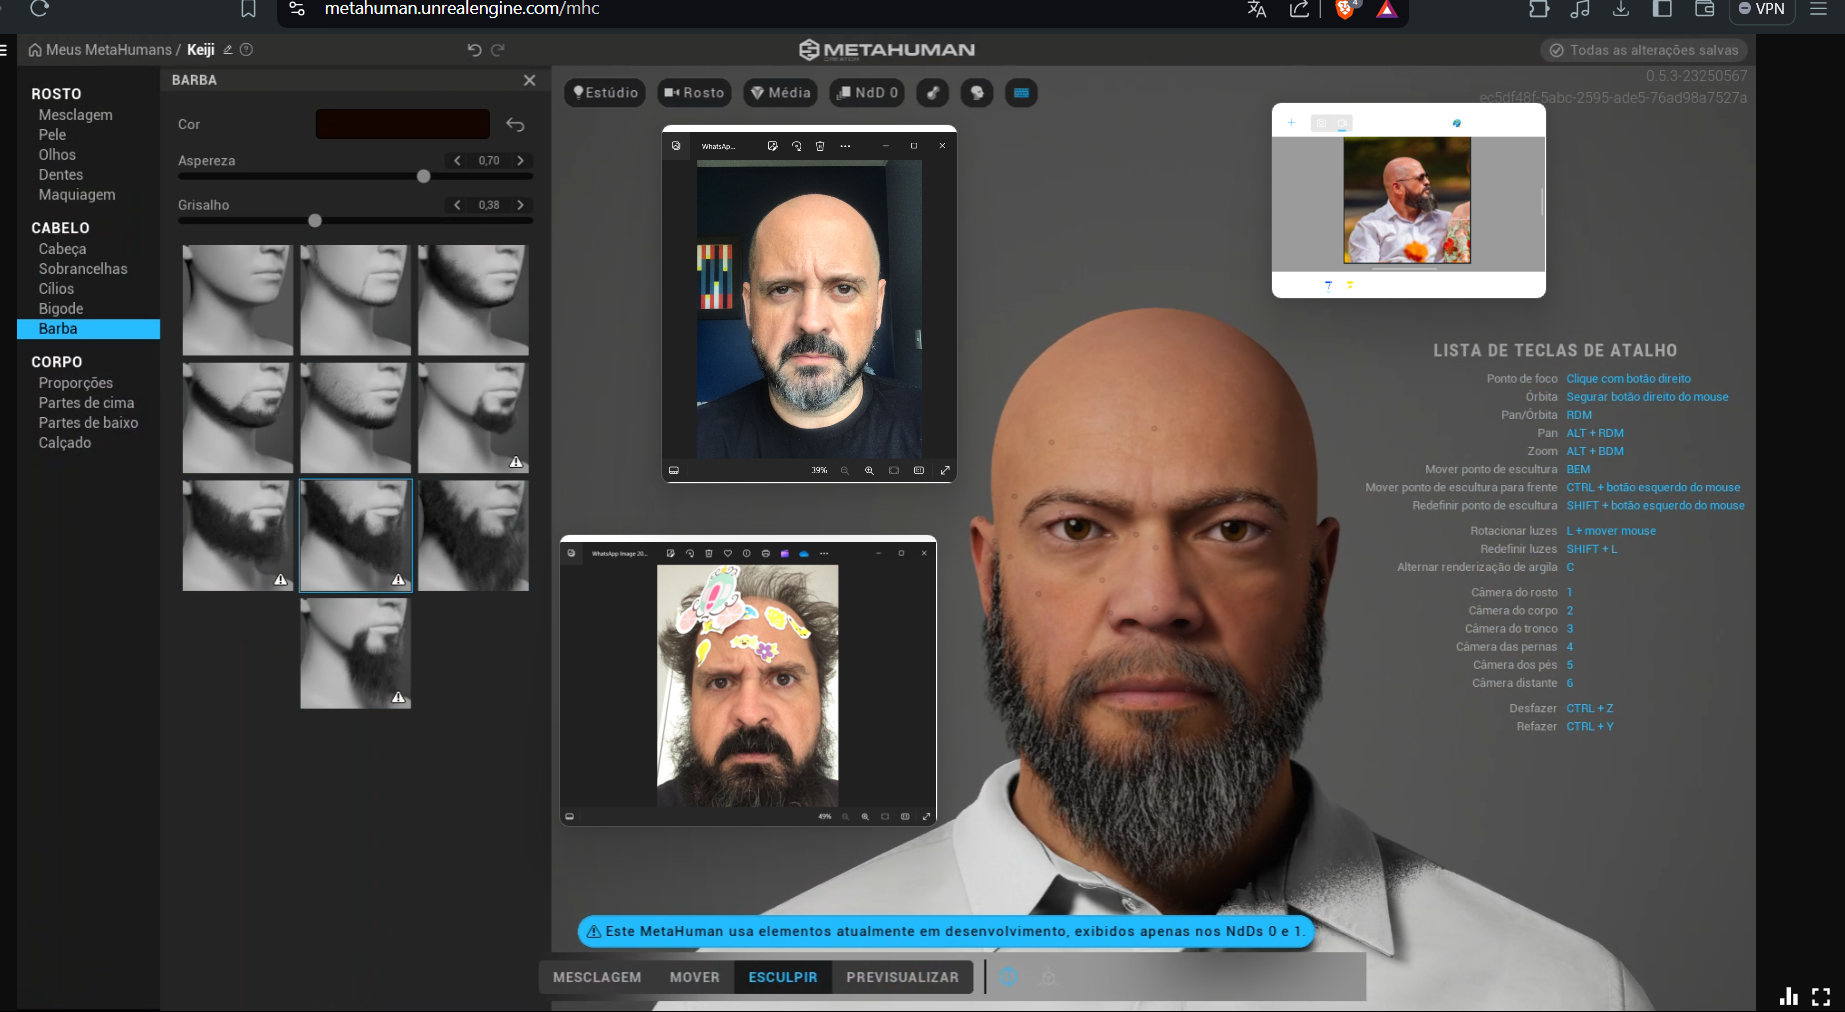
\includegraphics[height=8cm, keepaspectratio]{img/Metahuman.png}
    \caption{Captura de tela do MetaHuman creator. \\
        \textbf{Fonte:} Autoria Própria.}
    \label{fig:metahuman creator}
\end{figure}

Um aspecto fundamental para a integração convincente de Metahumans em ambientes virtuais é a animação. Cada \textit{MetaHuman} possui um "esqueleto digital" interno, uma estrutura articulada que permite a aplicação de movimentos, como mostrado na Figura \ref{fig:skeleton}. Através da importação de animações pré-definidas, que podem ser vistas na Figura \ref{fig:animacoes}, ou da criação de animações personalizadas utilizando softwares de animação 3D, é possível atribuir aos Metahumans ações como andar, correr, pular, gesticular e interagir com objetos no ambiente virtual. A fluidez e naturalidade dessas animações são essenciais para garantir a imersão do usuário e a credibilidade da representação.

\begin{figure}[H]
    \centering
    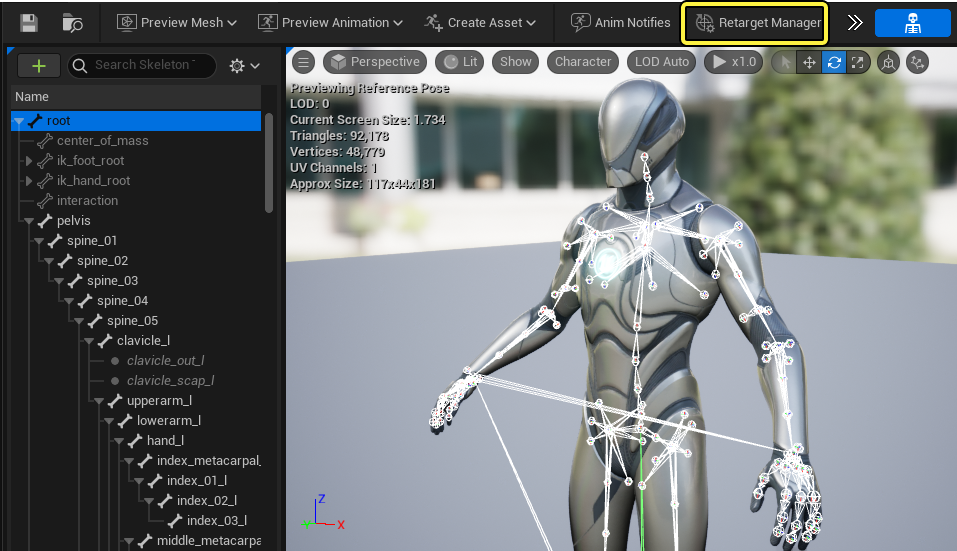
\includegraphics[height=8cm, keepaspectratio]{img/skeleton.png}
    \caption{Esqueleto digital.\\
        \textbf{Fonte:} Autoria Própria.}
    \label{fig:skeleton}
\end{figure}

\begin{figure}[H]
    \centering
    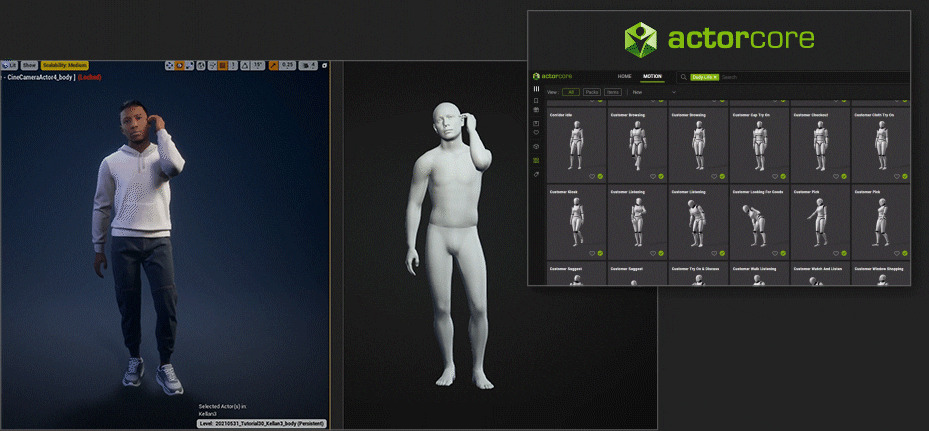
\includegraphics[height=8cm, keepaspectratio]{gif/animacoes/feature_body_motion-0000.jpg}
    \caption{ Print do pacote de animações Unreal.\\
        \textbf{Fonte:} Autoria Própria.}
    \label{fig:animacoes}
\end{figure}


A Figura \ref{fig:metahumanEdson} ilustra a aplicação da tecnologia MetaHuman na representação do Professor Edson, profissional da área de artes e entusiasta da arqueologia. O modelo digital, criado a partir de fotografias como referência, captura suas características físicas com fidelidade, demonstrando o potencial da ferramenta na criação de representações personalizadas. A utilização de um MetaHuman com a aparência do Professor Edson em uma experiência de Patrimônio Virtual permite, por exemplo, que ele atue como um guia virtual, conduzindo os usuários por um sítio arqueológico reconstruído, fornecendo explicações e respondendo a perguntas, criando assim uma experiência mais interativa e humanizada.

\begin{figure}[H]
    \centering
    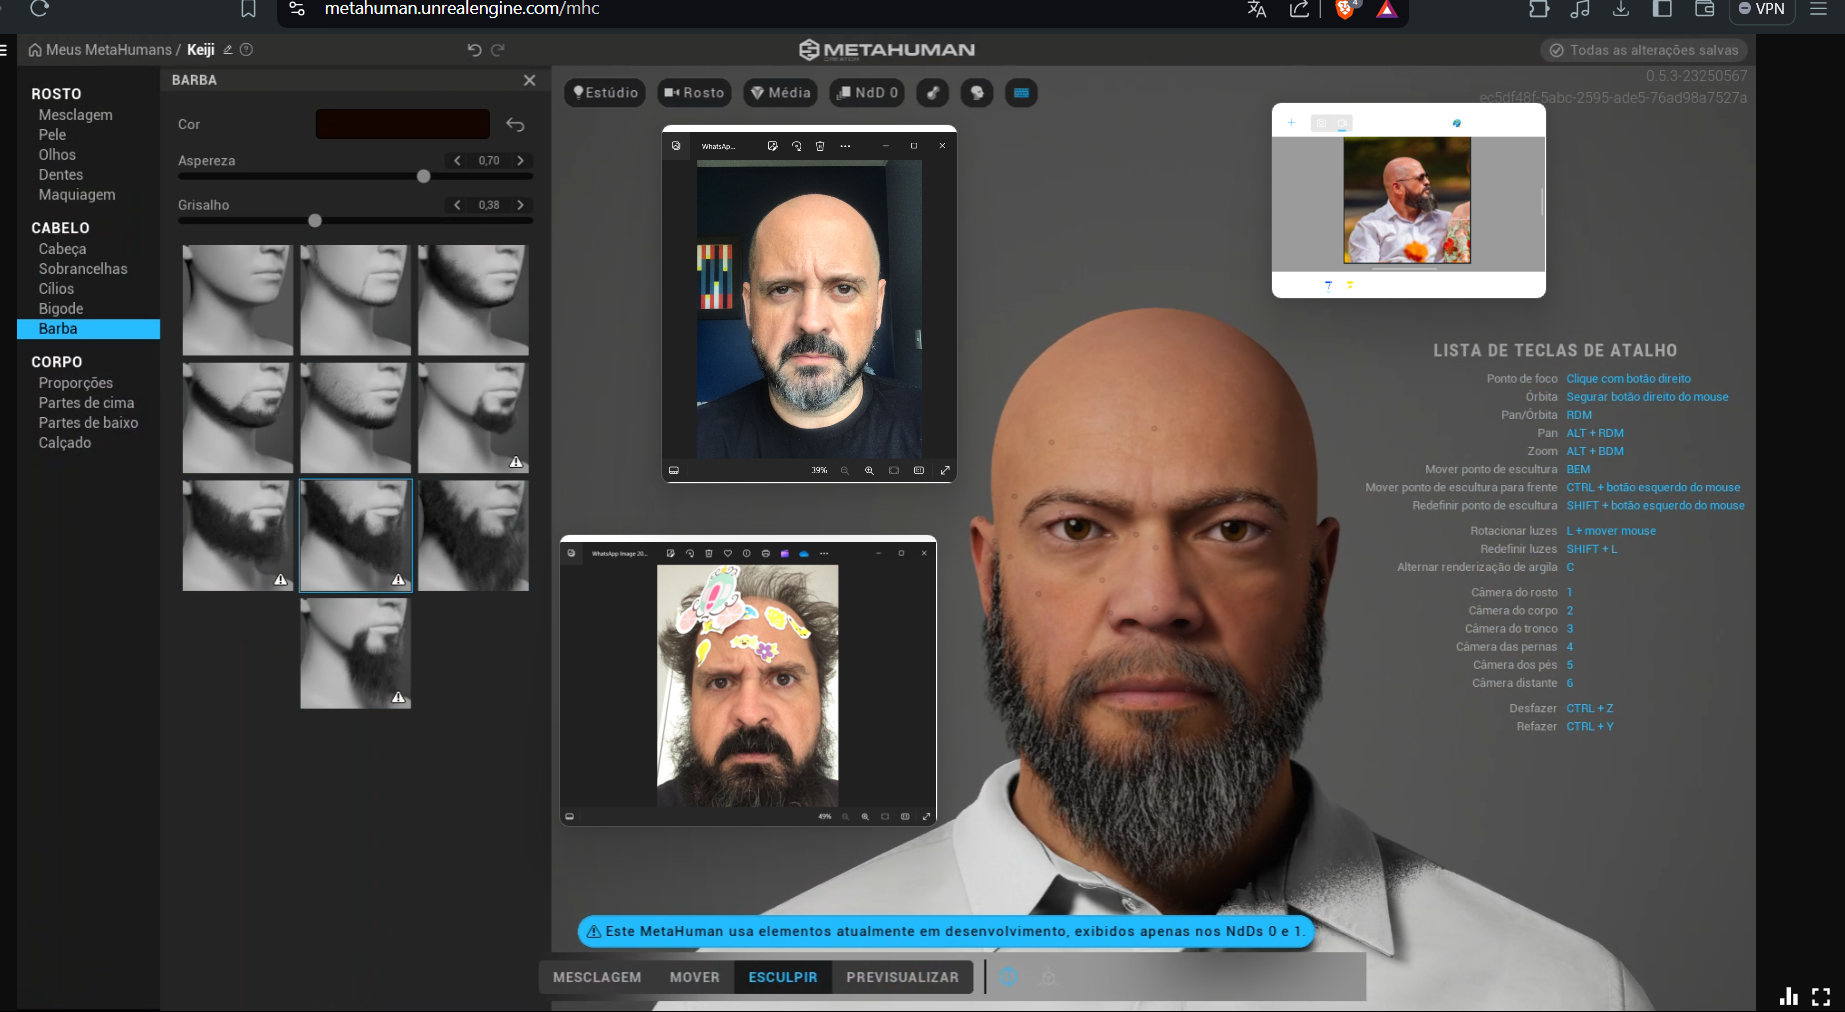
\includegraphics[height=8cm, keepaspectratio]{img/Metahuman.png}
    \caption{MetaHuman do professor Edson. \\
        \textbf{Fonte:} Autoria Própria.}
    \label{fig:metahumanEdson}
\end{figure}

A capacidade de gerar personagens virtuais realistas e personalizáveis, combinada com a possibilidade de animá-los de forma natural e convincente, torna os Metahumans uma ferramenta poderosa para a criação de experiências imersivas e envolventes no campo do Patrimônio Virtual. A presença de personagens virtuais humanoides pode contribuir significativamente para a comunicação de narrativas históricas.

\section{Engenharia de Software}
\subsection{Modelos de Processo}
Discutir diferentes modelos de processo de desenvolvimento de software, como Cascata, Agile, etc.

\subsection{UML: Unified Modeling Language}
A Unified Modeling Language (UML) é uma linguagem de modelagem amplamente utilizada para visualizar, especificar, construir e documentar artefatos de sistemas de software \citep{Booch2005}. Criada por Grady Booch, James Rumbaugh e Ivar Jacobson, a UML oferece um conjunto de diagramas padronizados que auxiliam no entendimento e na comunicação entre equipes de desenvolvimento. Segundo \cite{Booch2005}, a UML é composta por diagramas estruturais (como Diagramas de Classe e de Objetos) e comportamentais (como Diagramas de Caso de Uso e de Sequência), que permitem representar diferentes perspectivas de um sistema.

A UML tem sido fundamental para a engenharia de software, especialmente no contexto de desenvolvimento orientado a objetos. Conforme destacado por \cite{Fowler2005}, a linguagem é flexível o suficiente para ser adaptada a diferentes metodologias de desenvolvimento, como o Rational Unified Process (RUP) e métodos ágeis. Além disso, a UML é mantida e atualizada pela Object Management Group (OMG), garantindo sua evolução contínua para atender às necessidades da indústria de software \citep{OMG2017}.

\subsection{Cenário de Caso de Uso}
Descrever o que é um cenário de caso de uso e sua importância na definição de requisitos.

\subsection{Requisitos Funcionais}
Listar e explicar os requisitos funcionais do sistema a ser desenvolvido.

\subsection{Requisitos Não Funcionais}
Listar e explicar os requisitos não funcionais, como desempenho, segurança, usabilidade, etc.

\section{Desenvolvimento Web}
\subsection{Conceitos Básicos}
Definir o que é desenvolvimento web e a sua importância. Diferenciar entre front-end, back-end e full-stack development.

\subsection{Tecnologias Usadas}
Descrever as principais linguagens usadas, como HTML, CSS e JavaScript, além de frameworks como React, Angular e Vue.js. Comentar sobre linguagens e frameworks usados para o back-end, como Laravel, Django, Ruby on Rails, etc. Discutir tipos de bancos de dados, relacionais e não relacionais, e o uso de MySQL como exemplo.

\subsection{Experiência do Usuário (UX)}
A Experiência do Usuário (UX) é um conceito fundamental no design de sistemas interativos, focando na satisfação e na eficiência do usuário ao interagir com um produto ou serviço. Segundo \cite{Norman}, UX abrange todos os aspectos da interação do usuário com uma interface, desde a usabilidade até a experiência emocional.

\subsubsection{Heurísticas de Nielsen}
As heurísticas de Nielsen, propostas por Jakob Nielsen em 1994, são um conjunto de princípios amplamente utilizados para avaliar a usabilidade de interfaces. Essas heurísticas servem como diretrizes para identificar problemas de usabilidade e melhorar a interação do usuário. A seguir, são apresentadas as 10 heurísticas de Nielsen:

\begin{enumerate}
    \item \textbf{Visibilidade do Status do Sistema}: O sistema deve sempre manter os usuários informados sobre o que está acontecendo, por meio de feedback adequado e em tempo razoável. Por exemplo, barras de progresso ou mensagens de carregamento são formas de fornecer feedback.

    \item \textbf{Correspondência entre o Sistema e o Mundo Real}: O sistema deve falar a linguagem do usuário, com palavras, frases e conceitos familiares, em vez de termos técnicos. As informações devem aparecer em uma ordem natural e lógica.

    \item \textbf{Controle e Liberdade para o Usuário}: Os usuários frequentemente realizam ações por engano e precisam de uma "saída de emergência" claramente marcada para sair do estado indesejado. Isso inclui funcionalidades como "Desfazer" e "Refazer".

    \item \textbf{Consistência e Padrões}: Os usuários não devem se perguntar se palavras, situações ou ações diferentes significam a mesma coisa. Siga as convenções da plataforma e mantenha a consistência em todo o sistema.

    \item \textbf{Prevenção de Erros}: Um bom design evita que problemas ocorram. Isso pode ser feito eliminando condições propícias a erros ou verificando se há erros antes que o usuário confirme uma ação.

    \item \textbf{Reconhecimento em vez de Memorização}: Minimize a carga de memória do usuário, tornando objetos, ações e opções visíveis. O usuário não deve precisar lembrar informações de uma parte do sistema para outra.

    \item \textbf{Flexibilidade e Eficiência de Uso}: Aceleradores (como atalhos de teclado) podem aumentar a eficiência para usuários experientes, sem prejudicar a experiência de usuários iniciantes.

    \item \textbf{Estética e Design Minimalista}: As interfaces não devem conter informações irrelevantes ou raramente necessárias. Cada unidade extra de informação compete com as unidades relevantes e diminui sua visibilidade relativa.

    \item \textbf{Ajudar os Usuários a Reconhecer, Diagnosticar e Recuperar-se de Erros}: As mensagens de erro devem ser expressas em linguagem simples, indicar precisamente o problema e sugerir uma solução de forma construtiva.

    \item \textbf{Ajuda e Documentação}: Embora seja melhor que o sistema possa ser usado sem documentação, pode ser necessário fornecer ajuda e documentação. Essas informações devem ser fáceis de encontrar, focadas na tarefa do usuário e listar etapas concretas a serem seguidas.
\end{enumerate}

Essas heurísticas são amplamente utilizadas em avaliações de usabilidade, como inspeções heurísticas, para identificar problemas em interfaces e propor melhorias \citep{Nielsen1994}.

\subsubsection{Análise Heurística}
A \textbf{Análise Heurística} é um método de avaliação de usabilidade que consiste na inspeção sistemática de uma interface com base em um conjunto de princípios ou heurísticas predefinidas. Esse método é amplamente utilizado para identificar problemas de usabilidade em sites, aplicativos e outros sistemas interativos, sem a necessidade de envolvimento direto dos usuários.

\paragraph{Objetivos da Análise Heurística}
Os principais objetivos da análise heurística são:

\begin{itemize}
    \item Identificar problemas de usabilidade que possam prejudicar a experiência do usuário.
    \item Avaliar a conformidade da interface com princípios de design reconhecidos, como as heurísticas de Nielsen.
    \item Propor melhorias que aumentem a eficiência, a satisfação e a acessibilidade do sistema.
\end{itemize}

\paragraph{Etapas da Análise Heurística}
O processo de análise heurística geralmente envolve as seguintes etapas:

\begin{enumerate}
    \item \textbf{Seleção das Heurísticas}: Escolha um conjunto de heurísticas adequado ao contexto da avaliação, como as heurísticas de Nielsen ou Kanisaty.
    
    \item \textbf{Inspeção da Interface}: Um ou mais avaliadores examinam a interface, aplicando as heurísticas selecionadas para identificar problemas de usabilidade.
    
    \item \textbf{Documentação dos Problemas}: Cada problema identificado é documentado, descrevendo sua natureza, a heurística violada e, se possível, sugerindo uma solução.
    
    \item \textbf{Priorização e Relatório}: Os problemas são priorizados com base em sua gravidade e impacto na experiência do usuário, e um relatório detalhado é gerado para orientar as melhorias.
\end{enumerate}

\paragraph{Aplicações da Análise Heurística}
A análise heurística é aplicável em diversas situações, tais como:

\begin{itemize}
    \item Avaliação de protótipos durante o processo de design.
    \item Redesign de sites ou aplicativos existentes.
    \item Testes de usabilidade complementares, fornecendo insights adicionais.
\end{itemize}

Segundo \cite{Nielsen1994}, a análise heurística é uma das técnicas mais eficazes para identificar problemas de usabilidade de forma rápida e econômica, sendo amplamente utilizada por equipes de UX e design.

\subsection{Web Content Accessibility Guidelines (WCAG)}

As \textbf{Web Content Accessibility Guidelines (WCAG)}, desenvolvidas pelo \textbf{W3C}, são padrões globais para acessibilidade digital, garantindo que interfaces sejam acessíveis a todos, incluindo pessoas com deficiências \citep{wcag21}. Organizadas em quatro princípios (\textbf{POUR}), as WCAG abordam:

\begin{itemize}
    \item \textbf{Perceivable (Perceptível)}: Conteúdo deve ser apresentado de forma acessível (ex.: alternativas textuais para imagens).
    \item \textbf{Operable (Operável)}: Interfaces devem ser navegáveis por teclado e compatíveis com tecnologias assistivas.
    \item \textbf{Understandable (Compreensível)}: Conteúdo e operação devem ser claros e previsíveis.
    \item \textbf{Robust (Robusto)}: Conteúdo deve ser compatível com diversas tecnologias.
\end{itemize}

As WCAG possuem três níveis de conformidade: \textbf{A} (mínimo), \textbf{AA} (recomendado) e \textbf{AAA} (ótimo). Sua adoção promove inclusão digital, conformidade legal e melhoria da experiência do usuário \citep{wcag21}.

\subsection{Melhores Práticas}
Discutir a relevância da acessibilidade, otimização para SEO e práticas comuns de segurança em aplicações web.


\section{JAMstack e Desenvolvimento Web Moderno}
\label{sec:jamstack}
    % Explicar o conceito de JAMstack, vantagens, ferramentas (Next.js, Vercel, Headless CMS)


\section{Ferramentas Utilizadas}
\subsection{Visual Studio Code versão 1.88}
Descrever o uso do Visual Studio Code como editor de código, destacando suas funcionalidades como depuração, suporte a múltiplas linguagens e a extensão do Git.

\subsection{GitHub}
Contextualizar o uso do GitHub para controle de versão, explicando sua importância na gestão do código-fonte, colaboração com outros desenvolvedores e uso de funcionalidades como issues e merge requests.

\subsection{Notion}
Discutir como o Notion é utilizado para planejamento e organização do projeto, incluindo o uso do Kanban para gerenciamento de tarefas e prazos.

\subsection{Figma}
Descrever o uso do Figma para prototipação e design de interfaces, enfatizando suas funcionalidades colaborativas.


\subsection{Unreal Engine 5.4}
Descrever a escolha do Unreal Engine como plataforma para a criação de ambientes virtuais, discutindo suas capacidades de renderização.

\subsection{Agisoft Metashape versão}
Explicar como essas ferramentas são utilizadas para fotogrametria e geração de modelos 3D, discutindo suas funcionalidades.

\subsection{Reality Capture versão}
Explicar como essas ferramentas são utilizadas para fotogrametria e geração de modelos 3D, discutindo suas funcionalidades.

\subsection{Vercel}
falar das caracteristicas da hospedagem e etc

\subsection{Heurio}
A extensão \textbf{Heurio} é uma ferramenta desenvolvida para auxiliar na realização de análises heurísticas de sites e interfaces digitais. Disponível como uma extensão para navegadores, o Heurio permite que profissionais de UX apliquem as heurísticas de usabilidade de forma prática e organizada, identificando problemas de usabilidade e propondo melhorias.

\subsubsection{Funcionalidades do Heurio}
O Heurio oferece uma série de funcionalidades que facilitam a análise heurística, incluindo:

\begin{itemize}
    \item \textbf{Lista de Heurísticas Integrada}: A extensão inclui uma lista de heurísticas de usabilidade, como as de Nielsen, que podem ser selecionadas e aplicadas diretamente durante a avaliação da interface.
    
    \item \textbf{Anotações e Comentários}: O Heurio permite que o avaliador faça anotações e comentários sobre problemas identificados, associando-os às heurísticas correspondentes. Isso facilita a documentação e a comunicação dos resultados.
    
    \item \textbf{Captura de Tela}: A ferramenta permite capturar telas da interface sendo avaliada, facilitando a visualização e a referência aos problemas encontrados.
    
    \item \textbf{Relatórios Automatizados}: Após a análise, o Heurio gera relatórios automatizados que organizam as anotações, capturas de tela e heurísticas aplicadas. Esses relatórios podem ser exportados e compartilhados com a equipe.
    
    \item \textbf{Colaboração em Equipe}: O Heurio suporta a colaboração entre múltiplos avaliadores, permitindo que equipes trabalhem juntas na mesma análise e compartilhem insights.
\end{itemize}

\subsubsection{Aplicação do Heurio}
O Heurio é particularmente útil em projetos de \textit{redesign} de sites, avaliação de protótipos e testes de usabilidade. Ele pode ser utilizado por equipes de \gls{ux}, designers e desenvolvedores para garantir que as interfaces atendam aos princípios de usabilidade e proporcionem uma experiência positiva ao usuário. Além disso, a ferramenta é flexível o suficiente para ser adaptada a diferentes contextos e metodologias de avaliação.

A extensão Heurio é um exemplo de como a tecnologia pode ser utilizada para aprimorar práticas de UX, tornando a análise heurística mais acessível e eficiente \citep{Heurio2023}.

\subsection{Inno Setup}
Descrever a ferramenta Inno Setup para a criação de instaladores, discutindo como ela facilita a distribuição do software.


